% !TeX program = xelatex
\documentclass[letterpaper, 10pt, conference]{ieeeconf} 

\usepackage{amsmath}
\usepackage{amsfonts}
\usepackage{enumerate}
\usepackage{graphicx}
\usepackage{url}
\usepackage{polyglossia}
\usepackage{xltxtra}

\graphicspath{ {images/} }
\IEEEoverridecommandlockouts                          
\overrideIEEEmargins
\setmainfont{TH SarabunPSK}
\sloppy
\urlstyle{same}
\XeTeXlinebreaklocale "th"
\XeTeXlinebreakskip = 0pt plus 0pt

% \defaultfontfeatures{Scale=1}
% \setdefaultlanguage{thai}
% \newfontfamily{\thaifont}[Script=Thai]{TH SarabunPSK}

\newcommand{\bG}{
	\mathbb{G}
}

\newcommand{\bV}{
	\mathbb{V}
}

\newcommand{\bE}{
	\mathbb{E}
}

\title{
\huge \bf ระบบจำลองการทำงานของระบบบิทคอยน์ที่สามารถต่อขยายได้ \\
Exntensible Simulation Framework for Bitcoin
}

\author{\LARGE ณัฐพล ธนิตสุขการ และ ภารุจ รัตนวรพันธุ์ \\
ภาควิชาวิศวกรรมคอมพิวเตอร์ คณะวิศวกรรมศาสตร์ มหาวิทยาลัยเกษตรศาสตร์ \\
Email: nuttapon.t@ku.th, paruj.r@ku.th
}

\begin{document}

\maketitle
\thispagestyle{empty}
\pagestyle{empty}

\section{บทนำ}

ในยุคปัจจุบันเรามีการแลกเปลี่ยนสินค้า ซื้อของออนไลน์กันมากขึ้น แต่การโอนเงินข้ามประเทศหรือทำธุรกรรมข้ามประเทศนั้น มีขั้นตอนต้องยืนยันเยอะมาก จนในสุดท้ายแล้วได้เกิดระบบการแลกเปลี่ยนเงินออนไลน์แบบใหม่ขึ้นมา นั่นก็คือระบบสกุลเงินดิจิตัลที่พัฒนามาจากบล็อกเชนนั่นเอง ซึ่งบิทคอยน์หรือสกุลเงินดิจิตัลแรกของโลกนั้น ถูกสร้างขึ้นมาด้วยภาษาคอมพิวเตอร์ ไม่มีใครเป็นเจ้าของบิทคอยน์ ไม่มีรูปร่างและไม่สามารถจับต้องได้ โดยระบบของบิทคอยน์ ถูกรันโดยคอมพิวเตอร์ของผู้ใช้งานทั่วโลก โดยใช้ระบบซอฟต์แวร์ในการถอดสมการคณิตศาสตร์ โดยคุณสมบัติสำคัญของ บิทคอยน์คือ โปร่งใส่ 100\% กล่าวคือสามารถตรวจสอบรายการย้อนหลังได้ อีกทั้งยังมีความรวดเร็วและความปลอดภัยสูงมากอีกด้วย ระบบบิทคอยน์ประสบความสำเร็จอย่างมากในทางปฏิบัติ แต่ขาดทฤษฎีที่เข้มแข็งมารองรับทำให้การทำนายปัญหาที่จะเกิดขึ้นกับระบบทำได้ยาก ดังนั้นโครงงานนี้จึงมีส่วนช่วยอย่างมากในการจำลองการทำงานภายในของระบบบิทคอยน์ สามารถเห็นถึงโครงสร้างและปรากฏการณ์ต่างๆ ทำให้ง่ายต่อการศึกษาและพยากรณ์พฤติกรรมของบิทคอยน์ในอนาคต

\begin{itemize}
	\item {วัตถุประสงค์ของการศึกษา}
	\begin{itemize}
		\item เพื่อให้นิสิตมหาวิทยาลัยเกษตรศาสตร์ได้ทดลองใช้ระบบการแลกเปลี่ยนแบบสกุลเงินดิจิตัล ที่กำลังเป็นที่นิยม ณ ปัจจุบัน
		\item เป็นระบบสกุลเงินดิจิตัลที่เข้าใจง่ายและใช้งานง่าย
		\item สามารถใช้โหนดหลายๆโหนดมาช่วยกัน mine ช่วยกันต่อบล็อกเชนได้อย่างถูกต้อง
		\item มีการทำงานที่รวดเร็ว เนื่องจากเขียนด้วยภาษา Golang ซึ่งเหมาะอย่างมากในการทำงานในระบบแบบกระจาย (distributed system)
		\item เป็นฐานโค้ด (codebase) ที่มีความกระชับและปรับแต่งได้ง่าย กล่าวคือสามารถนำโมดูล (module) อื่นๆ เข้ามาต่อเข้าเพื่อขยายขอบเขตการทำงานได้ง่าย
	\end{itemize}
	\item {ขอบเขตของการทำโครงงาน}
	\begin{itemize}
		\item สามารถทำรายการได้อย่างถูกต้อง เช่น การโอนเงิน
		\item สามารถใช้เครื่องคอมพิวเตอร์มาขุด (Mining) เพื่อช่วยระบบยืนยันการทำรายการได้อย่างถูกต้อง
		\item สามารถใช้งานได้จริงในชีวิตประจำวัน
		\item ตัวระบบต้องมีความปอลดภัยสูง
	\end{itemize}
	\item {ประโยชน์ที่คาดว่าจะได้รับ}
	\begin{itemize}
		\item ได้ระบบสกุลเงินดิจิตัลที่ทำงานรวดเร็ว มีความเรียบง่าย และคล้ายคลึงกับระบบบิทคอยน์ที่ผู้คนทั่วโลกใช้งานอยู่ในขณะนี้
		\item สามารถใช้งานได้จริงในมหาวิทยาลัยเกษตรศาสตร์ เพื่อนิสิตจะได้สร้างความเคยชินกับระบบสกุลเงินเข้ารหัสที่จะเผชิญในอนาคต
		\item สามารถเป็นแบบอย่างให้แก่ผู้ที่สนใจในด้านบล็อกเชนและสกุลเงินเข้ารหัสนำไปต่อยอดต่อไปได้
		\item ได้นำความรู้หลากหลายสาขามาประยุกต์ใช้งานเข้าด้วยกัน ทั้งทางด้านวิทยาการเข้ารหัสลับ (Cryptography), ด้านเน็ตเวิร์กและด้านระบบการทำงานแบบกระจาย
	\end{itemize}
\end{itemize}

\section{ทฤษฎีที่เกี่ยวข้อง}

\subsection{บล็อกเชน (Blockchain)}
	บล็อกเชนคือรูปแบบการเก็บข้อมูลหรือเรียกว่าเป็นฐานข้อมูลแบบหนึ่งของระบบที่ไม่มีศูนย์กลางแต่เชื่อถือได้และโกงยาก กล่าวคือการให้ทุกคนถือเอกสารชุดเดียวกันคนละก๊อปปี้ด้วยวิธีแบบเพียร์ทูเพียร์ (Peer-to-Peer) ก็คือไม่ต้องมีคนตรงกลาง ทุกคนที่อยู่บนระบบเน็ตเวิร์คช่วยกันรันระบบ ซึ่งทำให้ระบบไม่มีทางล่มตราบใดที่ยังมีคนอยู่ในระบบเน็ตเวิร์คอยู่ ข้อมูลก็ไม่มีทางหายสาบสูญเพราะทุกคนช่วยกันถือไว้คนละชุด หากข้อมูลมีการเพิ่มขึ้นหรือมีบล็อกใหม่ ทุกคนในระบบเน็ตเวิร์คก็จะได้ข้อมูลใหม่ไปเพิ่มฐานข้อมูลในมือตัวเองด้วยกันทุกคน เมื่อมีการอัปเดตก็จะอัปเดตด้วยกัน โดยมั่นใจได้ว่าเอกสารเหล่านั้นเชื่อถือได้แน่นอนไม่มีการปลอมแปลง

	{\centering 
		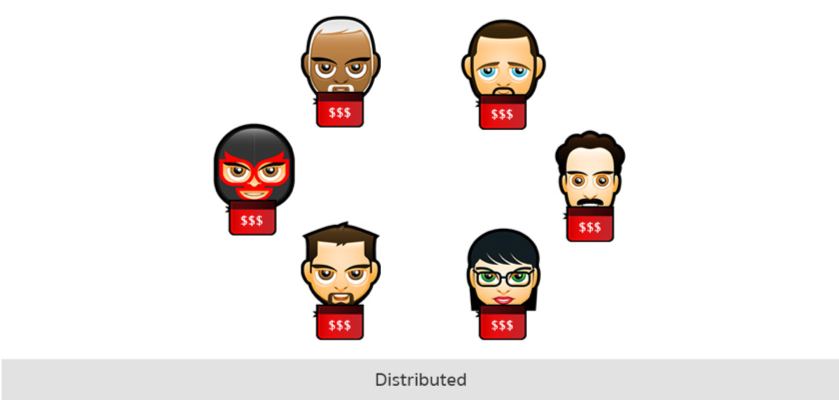
\includegraphics[scale=0.5]{related-work-1} \\
		ภาพที่ 1: ทุกคนถือข้อมูลของทั้งระบบเอาไว้คนละก็อปปี้ \par 
	}

\subsection{ศาสตร์การเข้ารหัสลับ (Cryptography)}

	\par เป็นสกุลเงินดิจิตัลที่ถูกพัฒนามาโดยหลักการสำคัญทาง Cryptography 2 หลักการหลักๆ คือ วิทยาการเข้ารหัสลับแบบคีย์สาธารณะ (public-key cryptography) และ แฮชฟังก์ชัน (hash function)
	วิทยาการเข้ารหัสลับแบบคีย์สาธารณะ ถูกนำมาใช้ทำเป็นกระเป๋าเงินและกุญแจรับเงิน คือ คีย์สาธารณะ (public key) และ คีย์ส่วนตัว (private key) ตามลำดับ
	แฮชฟังก์ชันหรือฟังก์ชันที่รับอินพุตขนาดใดๆเข้ามาและให้เอาต์พุตออกไปเป็นข้อความที่มีความยาวคงที่ เช่น 256 บิต ซึ่งมีคุณสมบัติสำคัญ 3 ประการที่จะถูกนำมาใช้ในเรื่องนี้ คือ
	\begin{enumerate}
		\item One-way function กล่าวคือ เราไม่สามารถทำย้อนกลับจากเอาต์พุตไปหาอินพุตได้
		\item Hiding property กล่าวคือ เราไม่สามารถรู้ส่วนใดส่วนหนึ่งของอินพุตได้จากเอาต์พุต
		\item Puzzle friendly กล่าคือ เราต้องใช้การออกแรง (brute force) เท่านั้น เพื่อที่จะได้มาซึ่งอินพุตที่เข้าคู่กับเอาต์พุตที่เราต้องการ
	\end{enumerate}
	\medskip

	{\centering 
		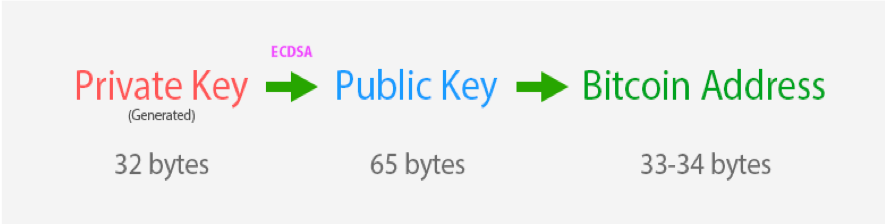
\includegraphics[scale=0.55]{related-work-2} \\
		ภาพที่ 2: การใช้วิทยาการเข้ารหัสลับแบบคีย์สาธารณะในระบบสกุลเงินดิจิตัล \par 
	}

\subsection{คอนเซนซัสแบบกระจาย (Distributed Consensus)}

	\par เป็นโปรโตคอลที่ใช้เพื่อการทำงานแบบกระจาย (decentralization) โดยการใช้เครือข่ายเพียร์ทูเพียร์ ให้แก่อาสาสมัครที่จะรับหน้าที่เก็บข้อมูลบัญชี (ledger) หรือบัญชีต่างๆบล็อกเชน โดยคอนเซ็นซัสแบบกระจาย (distributed consensus) มีวัตถุประสงค์หลักที่จะกระจายข้อมูลที่ถูกต้องไปยังโหนดต่างๆ และทำให้แน่ใจว่าทุกโหนดบนเน็ตเวิร์คบล็อกเชน มีรายการข้อมูลที่ถูกต้องและเหมือนกัน โดยมีหลักการทำงาน หลักๆดังนี้

	\begin{enumerate}
		\item คอยสอดส่องและสะสมรายการ ใหม่ๆที่ถูกปล่อยออกมา
		\item ตรวจสอบความถูกต้องของรายการนั้นๆ
		\item ส่งต่อรายการให้โหนด (node) ใกล้เคียง
	\end{enumerate}
	\medskip

	{\centering 
		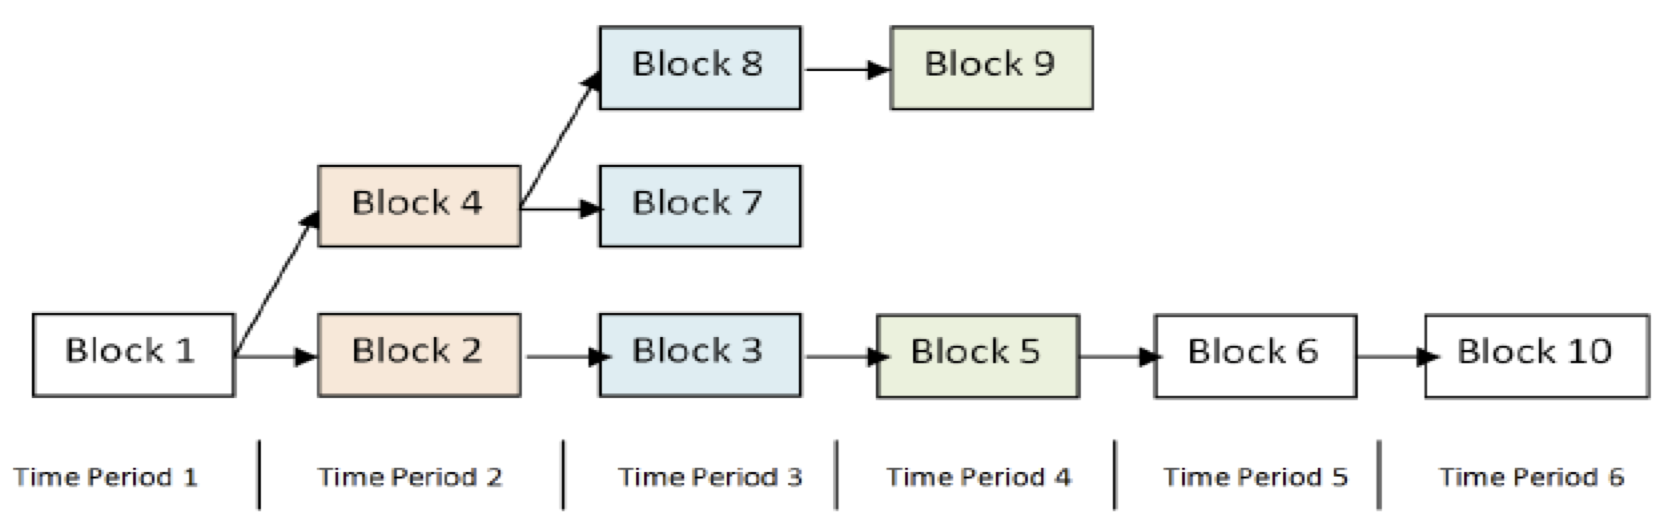
\includegraphics[scale=0.3]{related-work-3} \\
		ภาพที่ 3: ทุกคนจะยอมรับข้อมูลที่ถูกต้องและเหมือนกันในที่สุด \par 
	}

\section{รายละเอียดการพัฒนา}
\subsection{การออกแบบระบบ}
	ออกแบบ header fields ของระบบ มีขนาด 80 bytes ประกอบด้วย
	\begin{enumerate}
		\item version 4 bytes: เป็นตัวบอกว่าบล็อกนี้ ต้องทำตามกฏการยืนยันบล็อกแบบไหน
		\item previous block hash: ค่าแฮชของบล็อกก่อนหน้า
		\item merkle root hash: เป็นการทำดับเบิ้ลแฮชของต้นไม้ merkle ที่เก็บแฮชของ transaction ทั้งหมดในบล็อกนั้นไว้
		\item time: เป็นเวลาที่อยู่ในรูปของ unix timestamp ที่บล็อกนั้นๆเกิดขึ้นมา
		\item target bits: เป็นตัวกำหนดความยากของการ mine บล็อกนั้น ว่าต้องการค่าแฮชที่ต่ำกว่า target เท่าไหร่
		\item nonce: เป็นตัวเลขใดๆ ที่ถูกสุ่มขึ้นมาเพื่อให้แฮชรวมทั้งบล็อกต่ำกว่าค่า target ที่กำหนดไว้

	\end{enumerate}

	\par โดยแต่ละ block จะบรรจุ transaction หลายๆอันอยู่ภายใน ซึ่ง transaction แต่ละอันจะต้องระบุ input และ output เพื่อที่จะบอกว่าอ้างอิงเงินจาก transaction อะไร แล้วจะส่งเงินไปที่ transaction ไหนต่อไป \medskip

	{\centering 
		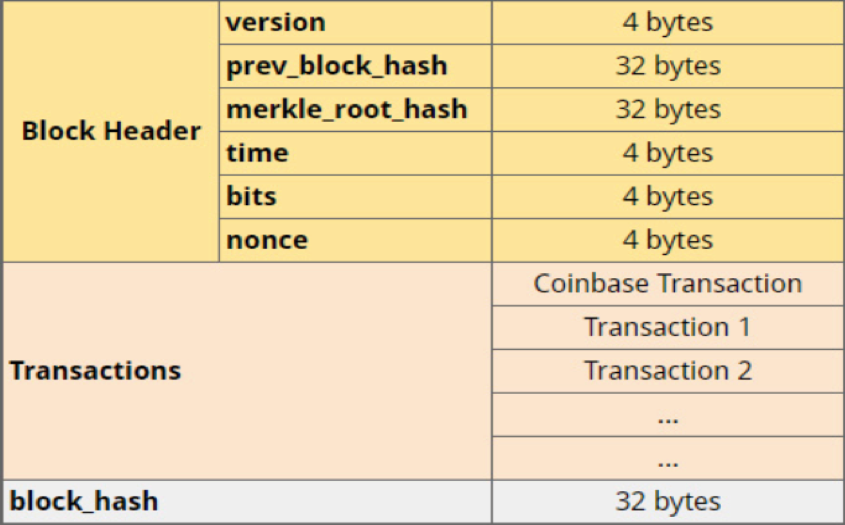
\includegraphics[scale=0.5]{system-detail-1} \\
		ภาพที่ 4: โครงสร้างของบล็อก \par 
	}
	\bigskip

	{\centering 
		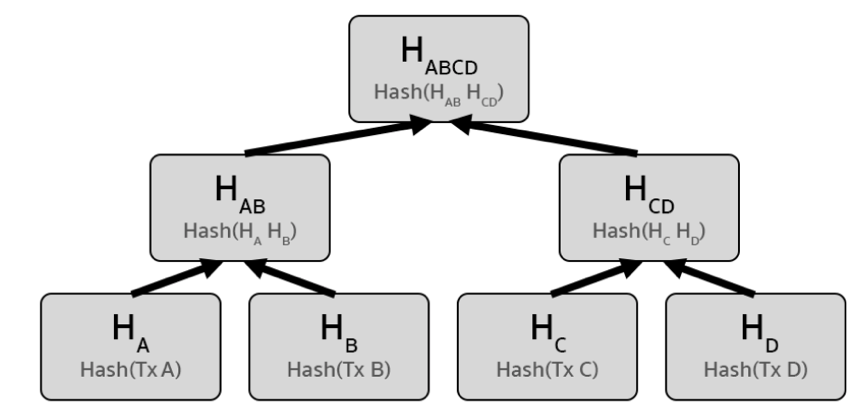
\includegraphics[scale=0.55]{system-detail-2} \\
		ภาพที่ 5: โครงสร้างของต้นไม้ merkle root \par 
	}
	\bigskip

	{\centering 
		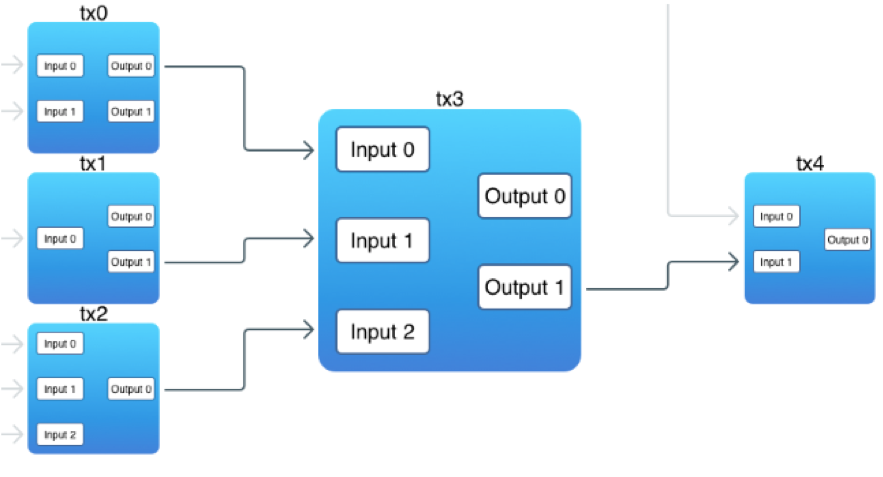
\includegraphics[scale=0.5]{system-detail-3} \\
		ภาพที่ 6: การอ้าง transaction input จาก transaction output ก่อนหน้า \par 
	}
	\bigskip
	
	\par โดยใช้หลักการของศาสตร์การเข้ารหัสลับที่ชื่อว่า Elliptic Curve Cryptography (ECDSA) ซึ่งเป็นหนึ่งในศาสตร์การเข้ารหัสโดยใช้คีย์สาธารณะ (Publick-key Cryptography) เป็นตัวรองรับความปลอดภัยของระบบ ECDSA จะสร้าง public key และ private key ที่เข้าคู่กันขนาด 512 bytes โดยมี public key เป็น Bitcoin address ซึ่งสามารถให้ผู้ใช้คนอื่น โอนเงินมาให้เราผ่านทางที่อยู่นี้ได้ และเก็บ private key ไว้เป็นตัวแทนความเป็นเจ้าของสมุดเล่มนี้ เพื่อใช้ในการถอนเงินหรือทำธุรกรรมต่างๆได้แต่เพียงผู้เดียว

	{\centering 
		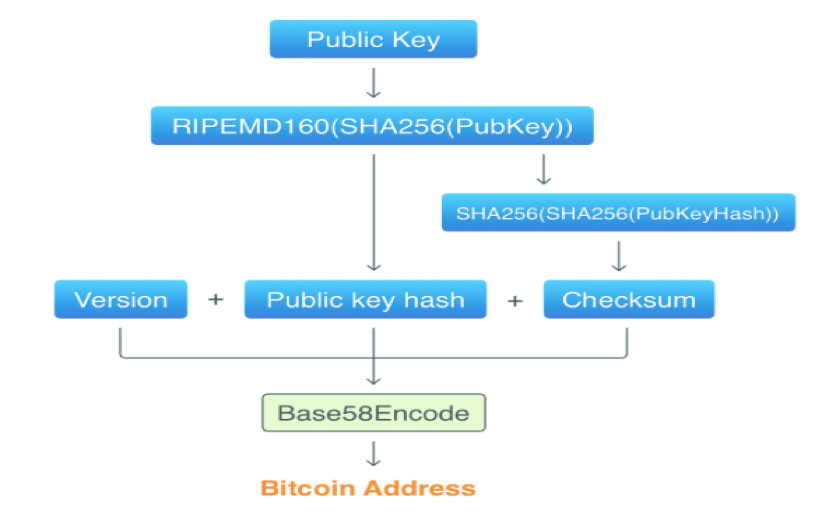
\includegraphics[scale=0.65]{system-detail-4} \\
		ภาพที่ 7: ขั้นตอนการสร้าง Bitcoin address จาก public key\par 
	}
	\bigskip

	\par การที่ผู้ใช้งานสามารถส่งต่อข้อมูลไปให้ผู้ใช้คนอื่นในระบบได้ผ่านการทำงานแบบเพียร์ทูเพียร์ (Peer-to-Peer) ได้มีการทำ cluster node membership, status dissemination และ failure detection เพื่อทำให้ระบบเพียร์ทูเพียร์เราเสถียรและป้องกันทนทานต่อความผิดพลาดได้ นอกจากนี้ยังทำ Atomic broadcast ด้วย TCP แทนที่จะใช้การ Broadcast/Multicast แบบปกติที่เป็น UDP ที่มีข้อเสียด้าน UDP Buffer Size ที่จะไม่รับรองการส่งข้อมูล เมื่อส่งข้อมูลขนาดใหญ่กว่า 512 bytes
	\par เมื่อผู้ใช้เยอะขึ้นมากๆ การส่งต่อ transaction, การส่งต่อบล็อก ย่อมก่อให้เกิดความไม่สอดคล้องกันได้ง่ายขึ้น เช่นบางกรณีนั้น ได้เกิดการแยกกันของบล็อกเชนเป็นสองสาย ซึ่งสุดท้ายจะถูกมองเป็นสายเดียวโดยยึดนโยบาย longest chain ตามบิทคอยน์โดย consensus Proof-of-Work ที่เราเลือกจะเป็นตัวการหลักในการจัดการปัญหานี้

\subsection{รายละเอียดของระบบ}
	\begin{enumerate}
		\item Core: ตัวส่วนหลักของระบบซึ่งมีพื้นฐานอยู่บนระบบเดียวกันกับ Bitcoin ซึ่งภายในจะมี public ledger เป็น blocks ต่อการเป็นสาย และในแต่ละ block จะบรรจุไปด้วย transaction ที่เก็บธุรกรรมของทุกคนในระบบที่ผ่านการยืนยันมาแล้วเอาไว้ 
		\item Proof-of-Work: ระบบมีการประยุกต์โปรโตคอลคอนเซนซัสหลากหลายรูปแบบ เพื่อทดสอบหาระบบที่ดีที่สุดที่จะนำมาใช้ในระบบจริงของมหาวิทยาลัยเกษตรศาสตร์ได้ เช่น Proof-of-Stake แต่เนื่องด้วยยังไม่มีการจัดการปัญหา Nothing-at-Stake และ LongRange-Attack ได้ จึงยังไม่ควรนำมาใช้จริงในระบบ สุดท้ายจึงได้เลือกใช้ตัว Proof-of-Work แบบเดียวกันกับ Bitcoin ซึ่งอาจจะมีปัญหาการกินทรัพยากรบ้าง แต่ก็เป็น consensus ที่เสถียรและนิยมกันมากที่สุดในขณะนี้
		\item Peer-to-Peer: มีการใช้งานระบบเพียร์ทูเพียร์ในรูปแบบของโปรโตคอลข่าวลือ (Gossip Protocol) ซึ่งเป็นวิธีการที่มีประสิทธิภาพมากที่สุดวิธีนึงที่มักจะถูกนำมาใช้ในระบบแบบกระจาย โดยในระบบได้มีการนำมาใช้เพื่อเป็นการสื่อสารกันระหว่างโหนด ให้โหนดได้คุยกัน เช่น ทำการกระจายหรือแลกเปลี่ยน transaction และ block กับโหนดที่อยู่ติดต่อ นอกจากโหนดต่างๆ จะต้องมีการทำส่งข่าวลือต่อๆกันแล้ว โหนดจำเป็นต้องมีการแพร่กระจายของสถานะโหนดข้างเคียงและแจ้งให้โหนดอื่นๆรู้ด้วย เราเรียกเหตุการณ์เช่นนี้ว่า status dissemination และโหนดต่างๆเหล่านี้มีโอกาสที่จะดับไปหรือมีโอกาสที่จะเป็นโหนดชั่วร้ายได้อีกตัว เราจึงจำเป็นต้องมีวิธีการจัดการในด้านนี้หรือที่เรียกว่า failure detection ในโปรโตคอลอีกด้วย
	\end{enumerate}

\subsection{ขั้นตอนการพัฒนา}
\begin{enumerate}
	\item ศึกษาการทำงานของระบบเหรียญดิจิตัล โดยศึกษาพื้นฐานต่างๆจาก e-book ของ Prince-ton University คือ Bitcoin and cryptocurrency technology ซึ่งมีหัวข้อสำคัญต่างๆ ดังนี้ 
	\begin{enumerate}
		\item เหตุผลที่เกิดเหรียญดิจิตัลขึ้นมาเพราะต้องการแก้ปัญหาการโอนเงินข้ามประเทศที่มีความล่าช้าเพราะขั้นตอนที่ยุ่งยากหรือมีการเก็บค่าธุรกรรมที่มากเกินจำเป็น
		\item การทำให้ทั่วโลกใช้เงินในสกุลเดียวกันเพื่อที่ในอนาคตจะเป็นโลกที่ไร้พรมแดนที่แท้จริง
		\item หลักการเข้าข้อมูลและการนำมาใช้ในการสร้างเหรียญดิจิตัล เพื่อให้มั่นใจว่าเราสามารถเชื่อถือในตัวเหรียญได้ว่ามีความปลอดภัยและมีความมั่นคงสูง
		\item เหรียญดิจิตัลตัวแรกของโลกซึ่งก็คือบิทคอยน์ ว่ามีโครงสร้างอย่างไรและทำอย่างไรถึงสามารถโอนเงินไปมาข้ามโลกได้โดยที่ไม่จำเป็นต้องมีศูนย์กลางของระบบ
		\item แมคคานิคซึ่มหลักของบิทคอยน์ว่ามีการทำงานอย่างไร ทั้งการทำ transaction และการต่อบล็อก 
	\end{enumerate}
	\item ศึกษาโปรโตคอลคอนเซนซัสที่ใช้ในการทำงานด้านระบบแบบกระจายหลายๆตัว เพื่อที่จะสามารถนำมาพิจารณาเลือกใช้ เช่น Proof of Work, Proof of Stake, Proof of Im-portance, Proof of Authority, Proof of Elapsed Time, Proof of Burn, Proof of Ca-pacity, Practical Byzantine Fault Tolerance, Tendermint Core, Loop Fault Tol-erance, Delegated Byzantine Fault Tolerance, Federated Byzantine Agree-ment, Paxos Consensus และ Raft Consensus
	\item ศึกษาจุดประสงค์และจุดเด่นของเหรียญดิจิตัลหลายๆสกุล เพื่อที่จะสามารถนำมาประยุกต์ใช้กับโครงงาน โดยมุ่งเน้นไปที่ความเร็วในการโอน, ความเป็นส่วนตัวของผู้ใช้, จำนวนบล็อกที่สามารถต่อได้ นอกจากนี้แต่ละเหรียญยังมีจุดประสงค์ที่แตกต่างกัน เช่น Ripple ร่วมมือกับธนาคารหลายแห่งทั่วโลก เพื่อที่จะต้องการเป็น Financial coin หรือ ZCash coin ที่เน้นที่ความเป็นส่วนตัวของผู้ใช้ หรือ ไม่สามารถตรวจสอบได้ และยังมีเหรียญที่เป็น Assets ที่ไป Contact กับเหรียญอื่น เช่น Ethereum , Waves, NEO เป็นต้น
	\item ศึกษาข้อดี-ข้อเสียของภาษาต่างๆ และดูความเหมาะสมของภาษาที่จะเอามาใช้ในงานจริง สุดท้ายจึงได้เลือกใช้ภาษา Go เพราะมีข้อดีที่เหมาะกับการทำ blockchain programming ในหลายๆด้าน เช่น
	\begin{enumerate}
		\item โค้ดที่เขียนในภาษา Go สามารถเข้าใจได้ง่ายและมีความสะอาด
		\item เร็วและมีสิทธิภาพสูง ไม่เหมือน Python ที่เป็น interpreted language แต่ Go เป็น compiled language เหมือนกับ C ซึ่งมีจุดเด่นเรื่องความเร็วเพราะมี over-head ตอนจัดการข้อผิดพลาดประเภท on-the-fly ได้ดี
		\item ถูกออกแบบมาเพื่อทำงานด้านระบบแบบกระจายได้ดี โดยสามารถเห็นได้จากซอร์ฟแวร์ดังๆหลายตัว เช่น Docker และ MongoDB ซึ่งถูกเขียนขึ้นมาจากภาษา Go แม้กระทั่ง Codebase ของ Ethereum และ Hyperledger ก็ถูกเขียนด้วยภาษา Go เช่นกัน
		\item Goroutines ที่สามารถทำงานด้านการเห็นพ้อง (concurrency) ได้อย่างมีประสิทธิภาพสูงสุด เนื่องจากการทำเทรด (thread) ด้วยภาษาโปรแกรมมิ่งอื่นๆ 1 เทรด อาจใช้แรมมากสุดถึง 1024 กิโลไบต์ แต่การใช้ Goroutines จะใช้แรมมากสุดไม่เกิน 4 กิโลไบต์
	\end{enumerate}
	\item ทำความเข้าใจเรื่องการโปรแกรมมิ่งบิทคอยน์จาก 3 assignments ที่มาจาก Bitcoin and Cryptocurrency Technology ของ Princeton University คือ
	\begin{enumerate}
		\item Scrooge Coin assignment จะให้สร้างการจัดการธุรกรรม (transaction han-dler) เพื่อให้สามารถยืนยันความถูกต้องของการทำธุรกรรม, หรือตรวจจับการทำธุรกรรมที่ไม่ถูกต้องเช่น double spending attack
		\item Consensus from Trust assignment โดยงานนี้เราจะได้รับกราฟความน่าเชื่อถือของโหนดแต่ละโหนดในระบบเน็ตเวิร์กมา โดยเรามีหน้าที่ต้องตรวจจับโหลดชั่วร้ายที่มีอยู๋ในระบบ
		\item Block Chain assignment เราจะต้องจัดการกับธุรกรรม โดยการนำไปเข้าบล็อก แล้วต่อไปอยู่บนบล็อกเชนจำลองได้
	\end{enumerate}
	\item ศึกษาตัวโค้ดหลักจาก https://github.com/bitcoin/bitcoin ซึ่งเป็นโค้ดจากระบบ บิทคอยน์หลัก เขียนด้วยภาษา C++  และบล็อกโพสของ Jeiwen เป็นแนวทางในการเขียนและออกแบบในรูปของภาษา Go
	\item ทำการทดสอบระบบทั้งหมด
	\item จัดทำเอกสารโครงงาน
\end{enumerate}

\section{ผลการพัฒนาโครงงาน}

\subsection{ผลการออกแบบและทดสอบระบบ}
	\begin{enumerate}
		\item ในส่วนของ Core จะได้หน้าต่างผู้ใช้งานที่สามารถทำหน้าที่ได้ครบถ้วนและเพียงพอต่อการใช้งาน
		\begin{itemize}
			\item createwallet ใช้สร้าง address ของกระเป๋าเงินใหม่
			\item showwallets ใช้สำหรับแสดงกระเป๋าเงินทั้งหมด
			\item printchain แสดงสถานะบล็อกเชนตั้งแต่ต้นจนถึงปัจจุบัน
			\item printpeer แสดง neighbor nodes
			\item reindexutxo จัดอินเด็กซ์การเก็บ unspent transaction ouput ใหม่
			\item send ทำการโอนเงินไปให้ address อื่นๆ
			\item checkupdate เป็นการ manual update สถานะของบล็อก
		\end{itemize}
		\medskip
		{\centering
			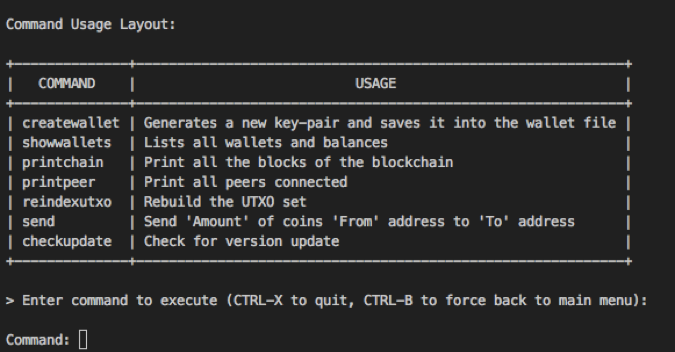
\includegraphics[scale=0.7]{result-1} \\
			ภาพที่ 8: หน้า User Interface \par
		}
		\medskip
		{\centering
			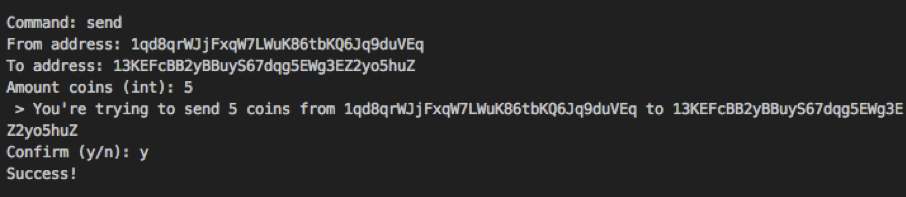
\includegraphics[scale=0.525]{result-2} \\
			ภาพที่ 9: ทดสอบการโอนเงิน \par
		}
		\medskip
		\item ในส่วนของ Web Visualization สามารถแสดงผลสถานะบล็อกปัจจุบันและรายละเอียดของแต่ละบล็อกได้เป็น tree ที่สวยงาม \\

		{\centering
			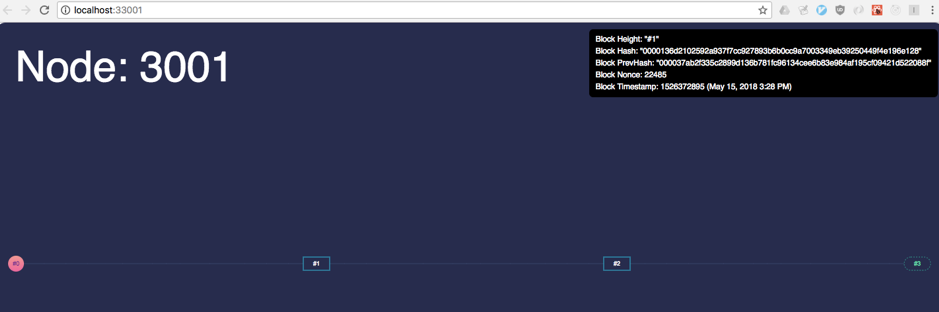
\includegraphics[scale=0.51]{result-3} \\
			ภาพที่ 10: หน้า Web Visualization \par
		}
	\end{enumerate}

\subsection{วิธีวัดผลและประเมินผล}
	\par การวัดและประเมินผล จะทดลองโดยการทำธุรกรรมจำนวนมหาศาลและมีโหนดที่ทำการยืนยัน transaction อยู่เยอะมากๆ เพื่อทดสอบดูว่าระบบจะเข้าสู่ consensus ได้ในที่สุด

\section{ผลการดำเนินโครงงานและวิจารณ์}

\subsection{สรุปผลการพัฒนาโครงงาน}
	ทั้งในส่วน Core และ Web Visualization สามารถทำงานและแสดงผลออกมาได้อย่างถูกต้อง
	\medskip

	\noindent
	สามารถทำรายการได้อย่างถูกต้อง เช่น การโอนเงิน 
	\hfill
	\textbf{[ผ่าน]} \\
	ระบบจะเข้าสู่คอนเซนซัสในที่สุด
	\hfill
	\textbf{[ผ่าน]} \\
	สามารถมีคนยืนยัน transaction ได้หลายคน
	\hfill
	\textbf{[ผ่าน]} \\
	ระบบมีความปลอดภัยจากการเกิด double spending
	\hfill
	\textbf{[ผ่าน]} \\
	ผู้ใช้ใหม่สามารถเข้าร่วมได้ตลอดเวลา
	\hfill
	\textbf{[ผ่าน]} \\
	มีเว็บวิชวลไลซ์สถานะบล็อกเชนของแต่ละผู้ใช้งาน
	\hfill
	\textbf{[ผ่าน]} \\
	โค้ดมีความกระชับ, สามารถเข้าใจและต่อยอดได้ง่าย 
	\hfill
	\textbf{[ผ่าน]} \\
	โครงงานสามารถนำไปใช้ได้จริง 
	\hfill
	\textbf{[ผ่าน]} \\

\subsection{ปัญหาและอุปสรรคในการดำเนินงาน}
	\begin{enumerate}
		\item ไม่สามารถทำงานให้เสร็จได้ตามแผนที่วางไว้ เนื่องจากงานในบางส่วนกินเวลามากกว่าที่คาดไว้
		\item มีไลบราลี่ให้เลือกใช้งานน้อยมาก เนื่องจากเป็นฟิลด์ที่ยังใหม่และเลือกใช้ภาษาที่มีเครื่องมือสำเร็จรูปยังไม่มากพอ
		\item ในส่วนของโค้ดหลัก ยังขาดการทำคู่มือการใช้งานเพื่อเพิ่มความง่ายให้นำไปใช้ต่อได้
	\end{enumerate}

\subsection{ข้อเสนอแนะในการพัฒนาต่อไป}
	\begin{enumerate}
		\item สามารถนำไปต่อยอดเป็นระบบจำลองการทำงานเพื่อตรวจจับอัตราการเกิดบล็อกกำพร้าในระบบบิทคอยน์ ซึ่งจะมีส่วนช่วยอย่างมากในการทำนายพฤติกรรมบางอย่างของระบบ
		\item ใช้ระบบการจำลองนี้เป็นโค้ดพื้นฐาน ในการใช้ต่อยอดบนระบบสกุลเงินดิจิตัลอื่นๆ เช่น Ethereum เพื่อทำการจำลองและทำนายพฤติกรรมได้เช่นเดียวกัน
	\end{enumerate}

\section*{เอกสารอ้างอิง}
	\begin{enumerate}[ {[}1{]} ]
		\item Bitcoin and Cryptocurrency technologies, \url{https://d28rh4a8wq0iu5.cloudfront.net/bitcointech/readings/princeton_bitcoin_book.pdf}, 
		[สืบค้นเมื่อ มกราคม 2561]
		\item Understanding Blockchain Consensus Models, \url{https://www.persistent.com/wp-content/uploads/2017/04/WP-Understanding-Blockchain-Consensus-Models.pdf?pdf=Understanding-Blockchain-Consensus-Models},
		[สืบค้นเมื่อ มกราคม 2561]
		\item Blockchain DIY with Python, \url{https://clumdee.github.io/blockchain-DIY-with-python}, 
		[สืบค้นเมื่อ มกราคม 2561]
		\item Blockchain for Geek, \url{https://nuuneoi.com/blog/blog.php?read_id=900},
		[สืบค้นเมื่อ กุมภาพันธ์ 2561]
		\item Go by Example, \url{https://gobyexample.com}, 
		[สืบค้นเมื่อ กุมภาพันธ์ 2561]
		\item Blockchain programming with Go, \url{https://jeiwan.cc},
		[สืบค้นเมื่อ กุมภาพันธ์ 2561]
		\item Consensus protocol for Blockchain, \url{https://nuuneoi.com/blog/blog.php?read_id=933}, 
		[สืบค้นเมื่อ มีนาคม 2561]
	\end{enumerate}

\end{document}
